\section{Results for Architecture 0 (Transformer Baseline)}
\label{sec:transformer-baseline-results}

This section presents the comprehensive experimental results for our Multi-Head mDeBERTa baseline architecture. We evaluate the model's performance across different classification thresholds and provide detailed analysis of its effectiveness for hierarchical narrative classification across multiple languages.

\subsection{Experimental setup and evaluation metrics}

Our evaluation was conducted on the development set comprising 178 documents across five languages (Bulgarian, English, Hindi, Portuguese, and Russian). The model was trained using a threshold of 0.65, and we systematically evaluated performance at four different classification thresholds: 0.5, 0.65 (training baseline), 0.7, and 0.8.

\subsection{Overall performance analysis}

\subsubsection{Threshold sensitivity analysis}

Table~\ref{tab:threshold-comparison} presents the comprehensive performance comparison across all tested thresholds for both narrative and subnarrative classification tasks.

\begin{table}[htbp]
\centering
\caption{Performance comparison across different classification thresholds. The training threshold (0.65) serves as the baseline for comparison.}
\label{tab:threshold-comparison}
\begin{tabular}{lcccccc}
\toprule
\multirow{2}{*}{\textbf{Threshold}} & \multicolumn{3}{c}{\textbf{Narratives}} & \multicolumn{3}{c}{\textbf{Subnarratives}} \\
\cmidrule(lr){2-4} \cmidrule(lr){5-7}
& \textbf{F1 Macro} & \textbf{F1 Micro} & \textbf{F1 Samples} & \textbf{F1 Macro} & \textbf{F1 Micro} & \textbf{F1 Samples} \\
\midrule
0.5 & 0.1800 & 0.2614 & 0.2475 & 0.0654 & 0.0987 & 0.0971 \\
\textbf{0.65*} & \textbf{0.2004} & \textbf{0.3145} & \textbf{0.2901} & 0.0776 & 0.1427 & 0.1543 \\
0.7 & 0.1825 & 0.2911 & 0.2657 & \textbf{0.0821} & 0.1516 & 0.1566 \\
0.8 & 0.0937 & 0.2012 & 0.2233 & 0.0583 & \textbf{0.1574} & \textbf{0.1750} \\
\bottomrule
\end{tabular}
\end{table}

The results reveal distinct performance patterns between narrative and subnarrative classification:

\paragraph{Narrative classification.} The training threshold of 0.65 consistently achieves the best performance across all metrics for narrative classification. This demonstrates excellent model calibration during training, with our primary metric F1 Samples reaching 0.2901, alongside F1 Macro of 0.2004 and F1 Micro of 0.3145. Lower thresholds (0.5) result in too many false positives, reducing the F1 Samples score by approximately 8.4\%. Conversely, very high thresholds (0.8) are overly conservative, leading to a substantial 23\% reduction in F1 Samples performance as the model misses many true positive predictions.

\paragraph{Subnarrative classification.} Most importantly for our primary F1 Samples metric, subnarrative classification significantly benefits from higher thresholds than the training baseline. Threshold 0.8 achieves the best F1 Samples performance (0.1750, representing a +13.4\% improvement over the training threshold), while also excelling in F1 Micro (0.1574, +10.3\% improvement). Threshold 0.7 provides the best F1 Macro (0.0821, +5.9\% improvement). This pattern suggests that more conservative predictions are particularly beneficial for fine-grained classification when evaluated on a per-document basis, likely because they reduce false positives in the challenging task of distinguishing between subtle subnarrative categories.

\begin{figure}[htbp]
    \centering
    \begin{subfigure}[b]{0.48\textwidth}
        \centering
        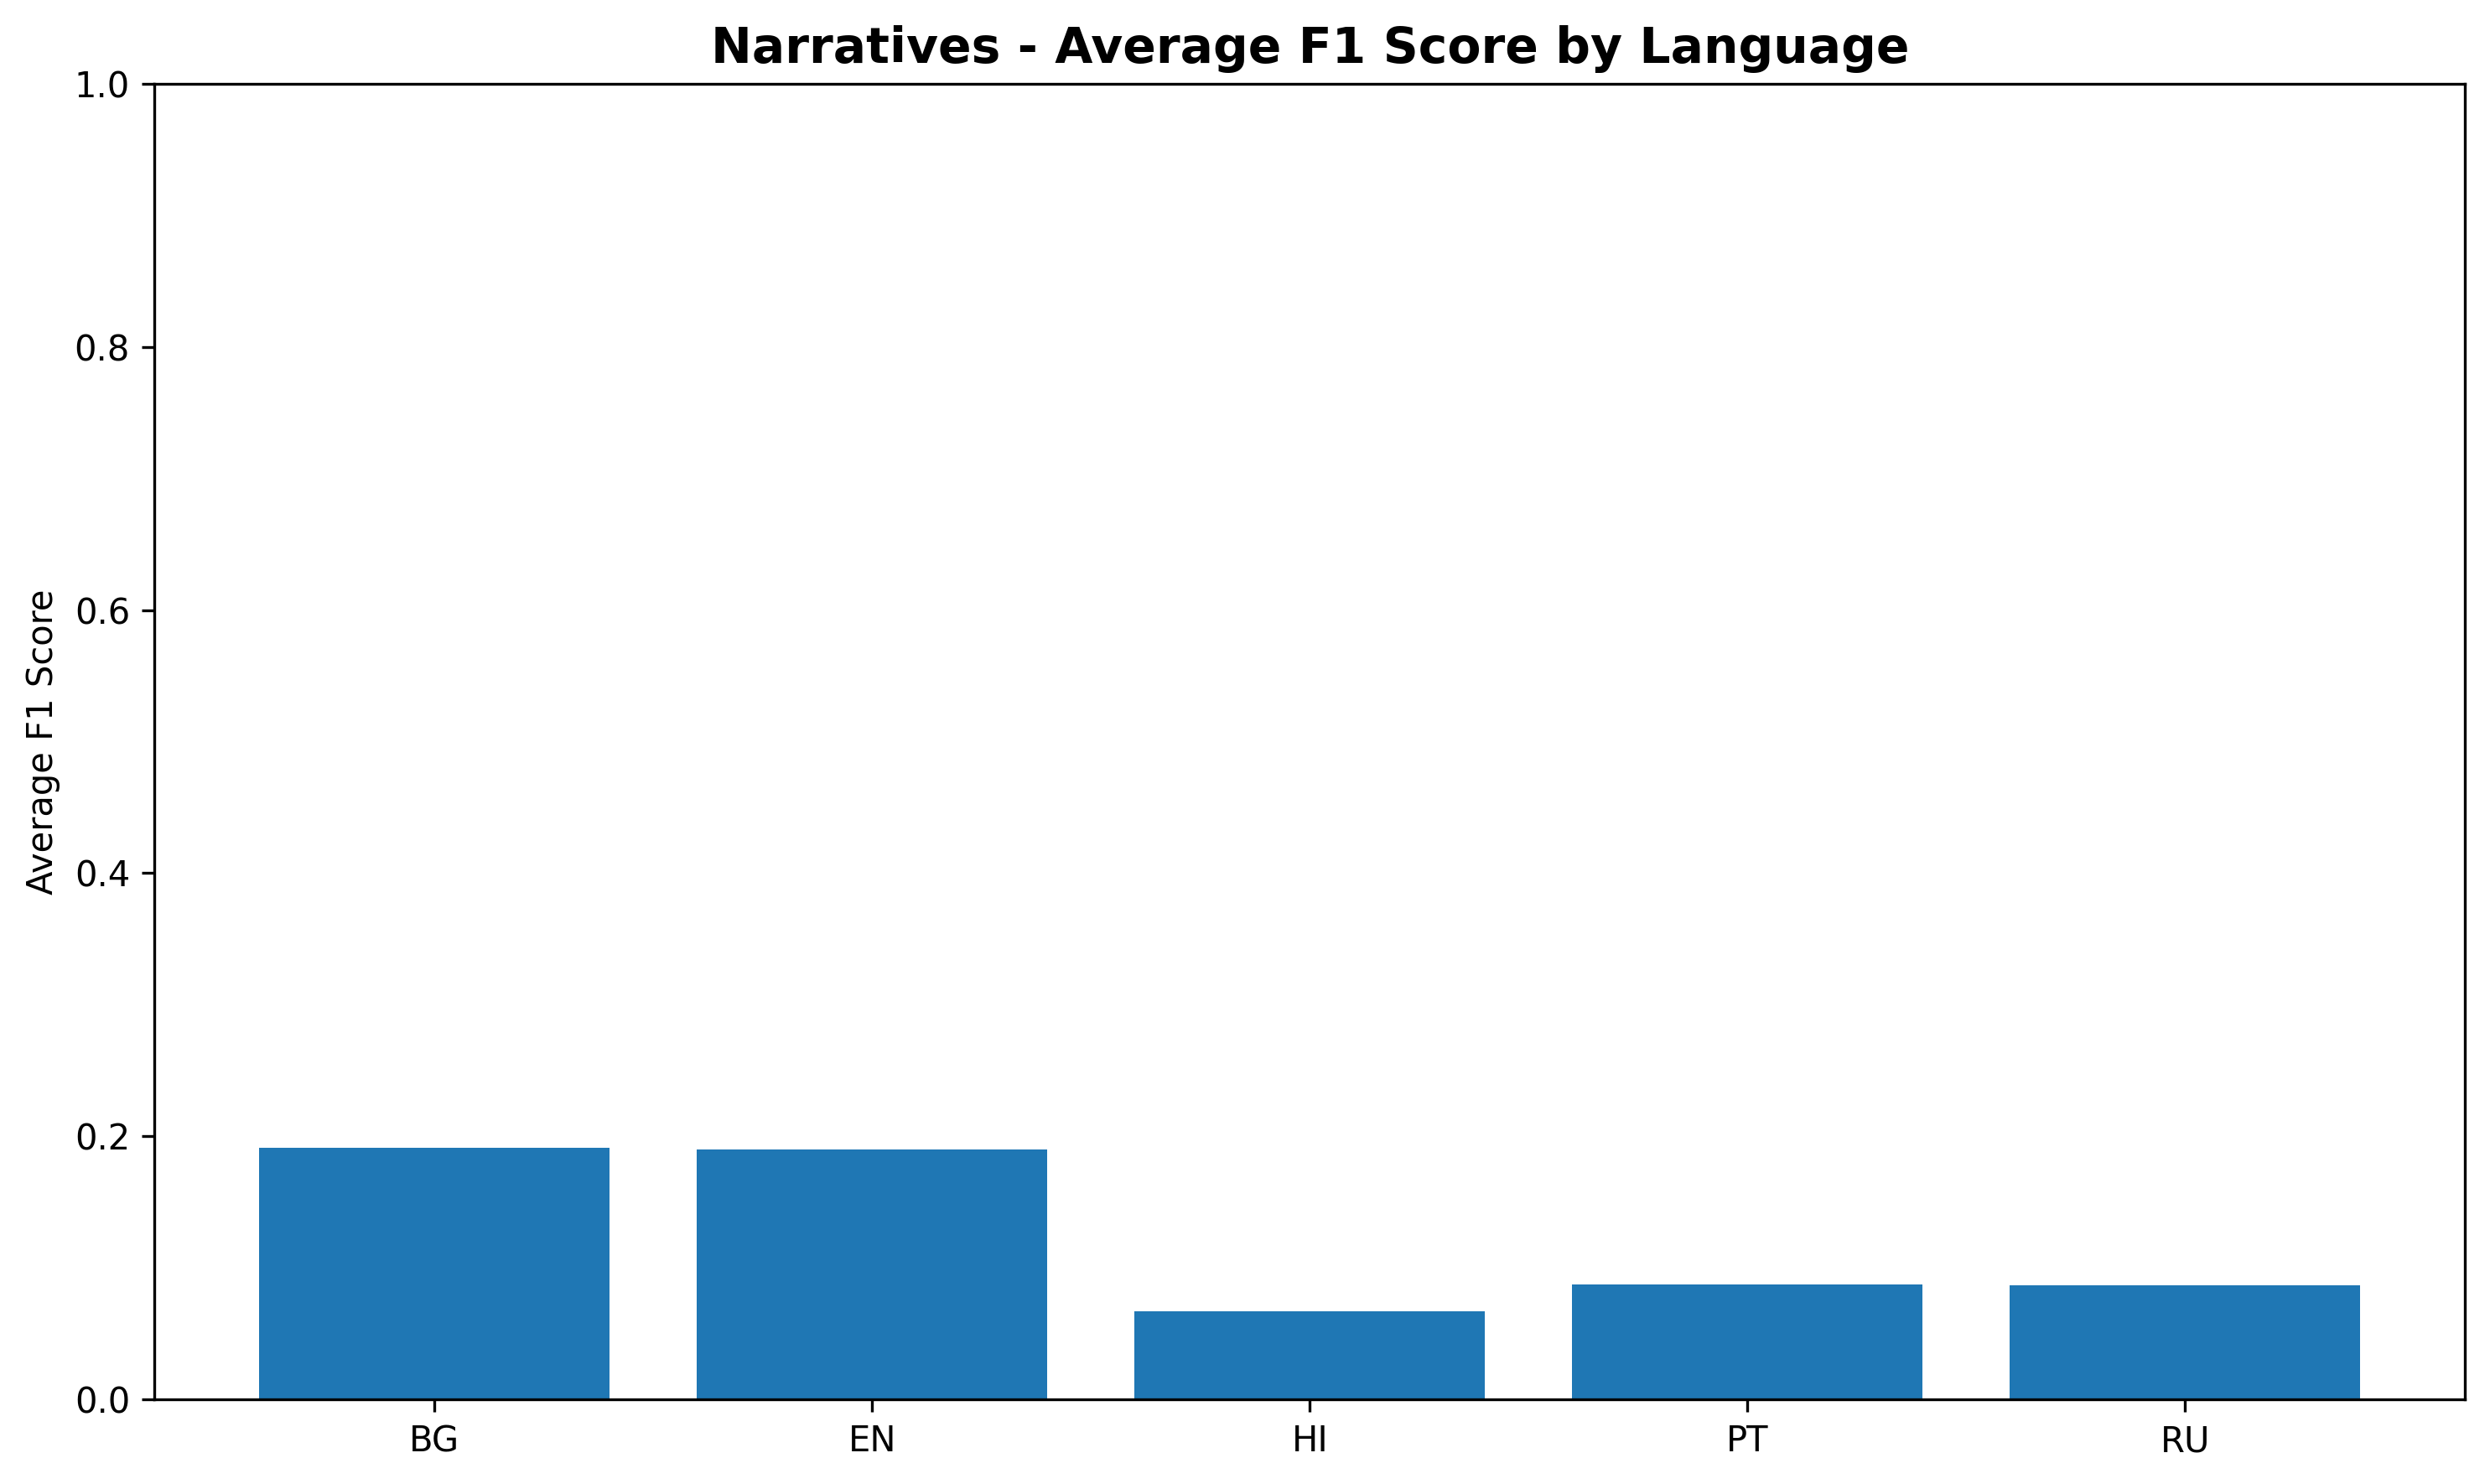
\includegraphics[width=\textwidth]{images/threshold_analysis/plots/narratives/f1_score_by_language.png}
        \caption{Narrative F1 scores by language}
        \label{fig:narratives-by-language}
    \end{subfigure}
    \hfill
    \begin{subfigure}[b]{0.48\textwidth}
        \centering
        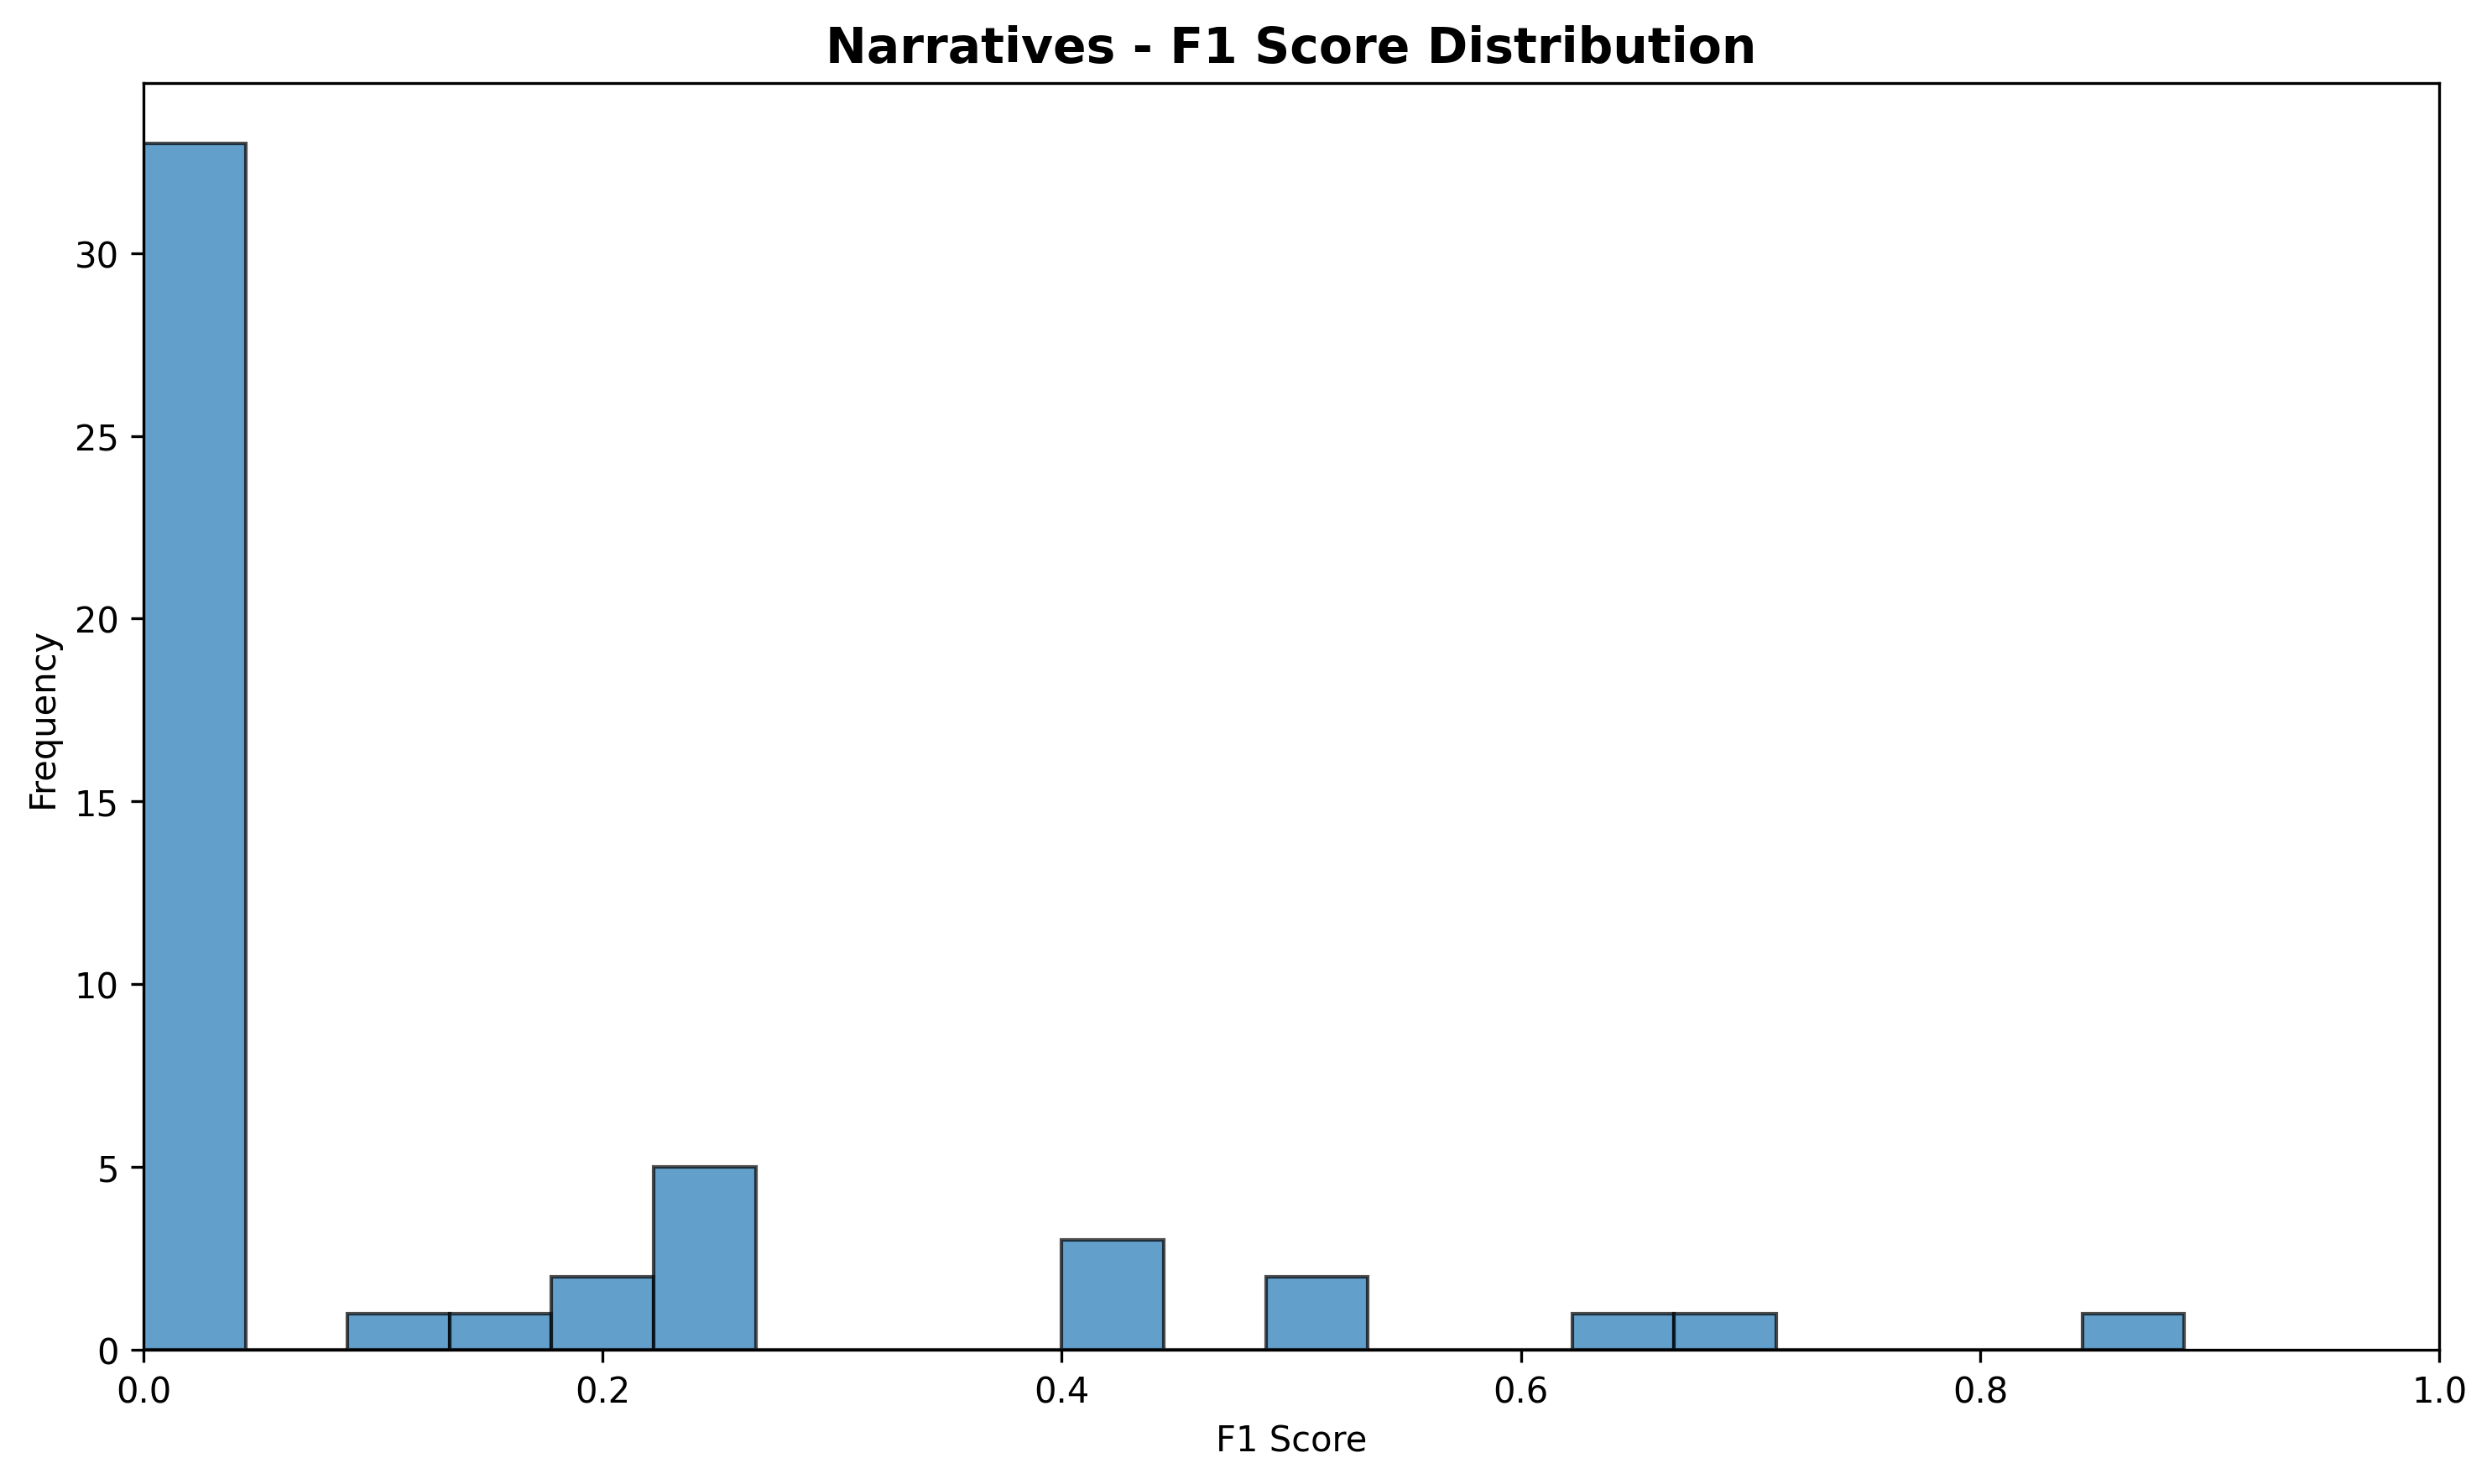
\includegraphics[width=\textwidth]{images/threshold_analysis/plots/narratives/f1_score_distribution.png}
        \caption{Narrative F1 score distribution}
        \label{fig:narratives-distribution}
    \end{subfigure}
    \caption{Narrative classification performance analysis at optimal threshold (0.65). (a) shows language-specific performance variations, with Portuguese achieving the highest F1 scores. (b) displays the distribution of F1 scores across all narrative categories, revealing the challenge of class imbalance.}
    \label{fig:narratives-detailed-analysis}
\end{figure}

\begin{figure}[htbp]
    \centering
    \begin{subfigure}[b]{0.48\textwidth}
        \centering
        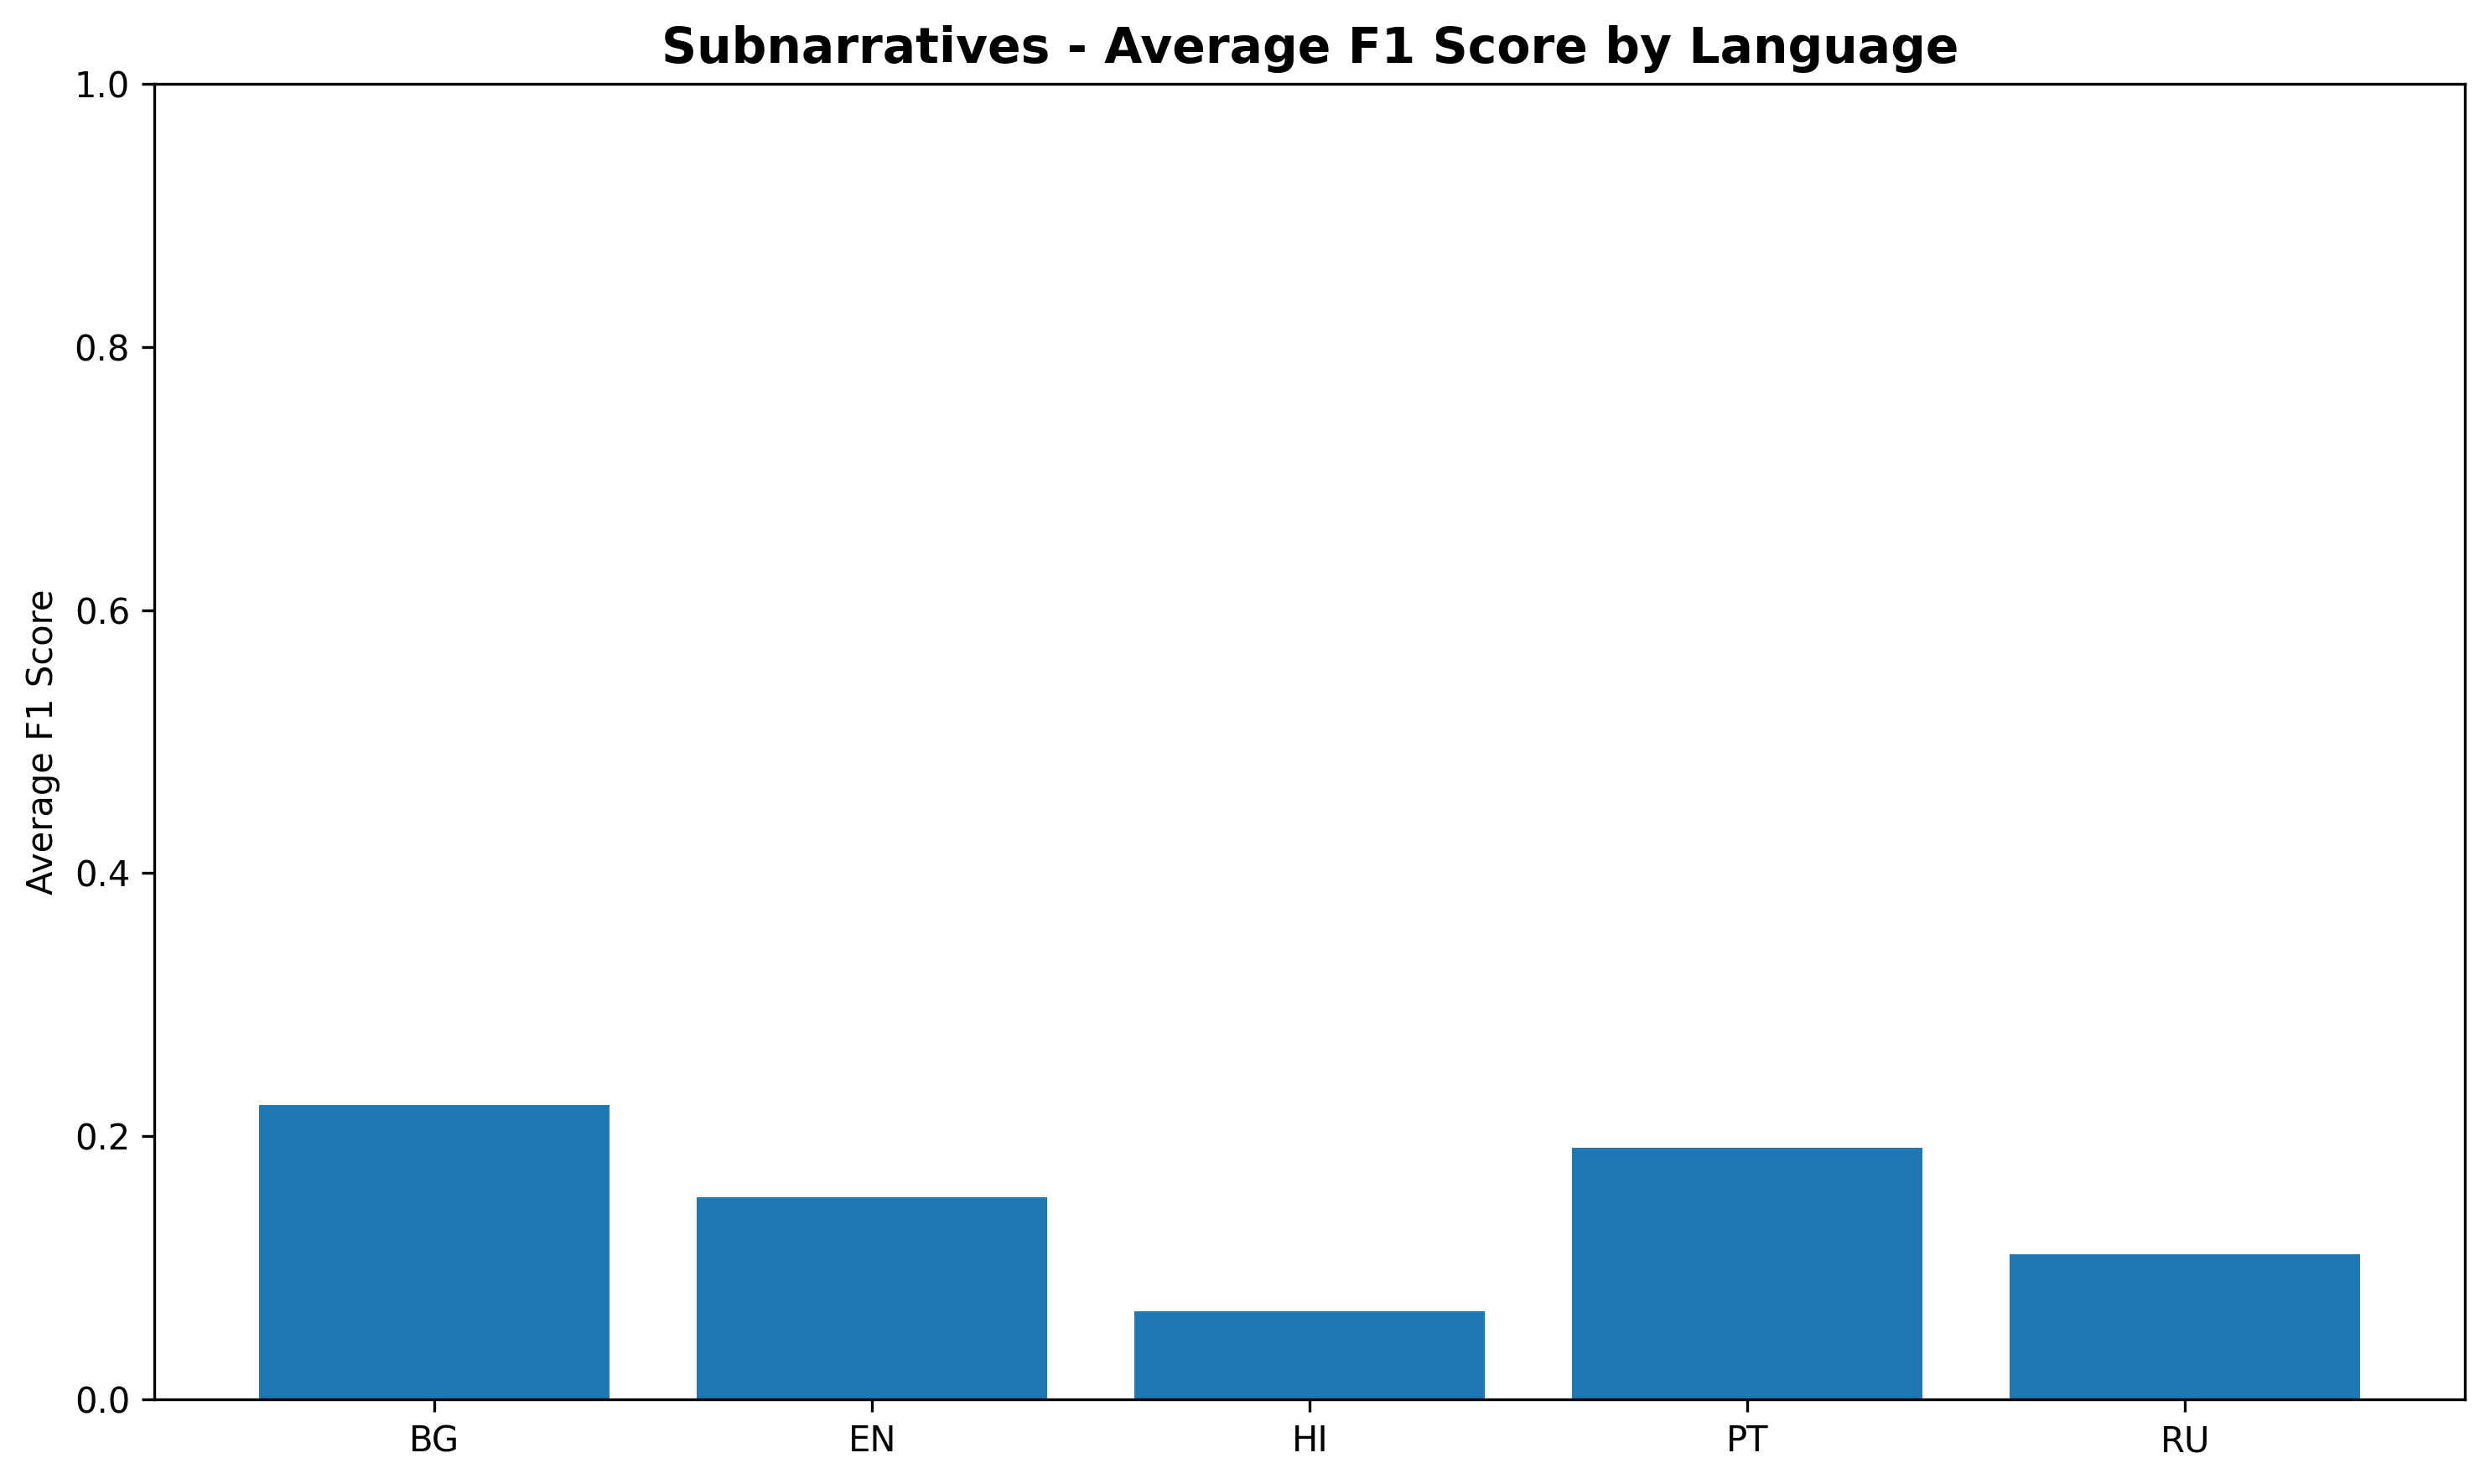
\includegraphics[width=\textwidth]{images/threshold_analysis/plots/subnarratives/f1_score_by_language.png}
        \caption{Subnarrative F1 scores by language}
        \label{fig:subnarratives-by-language}
    \end{subfigure}
    \hfill
    \begin{subfigure}[b]{0.48\textwidth}
        \centering
        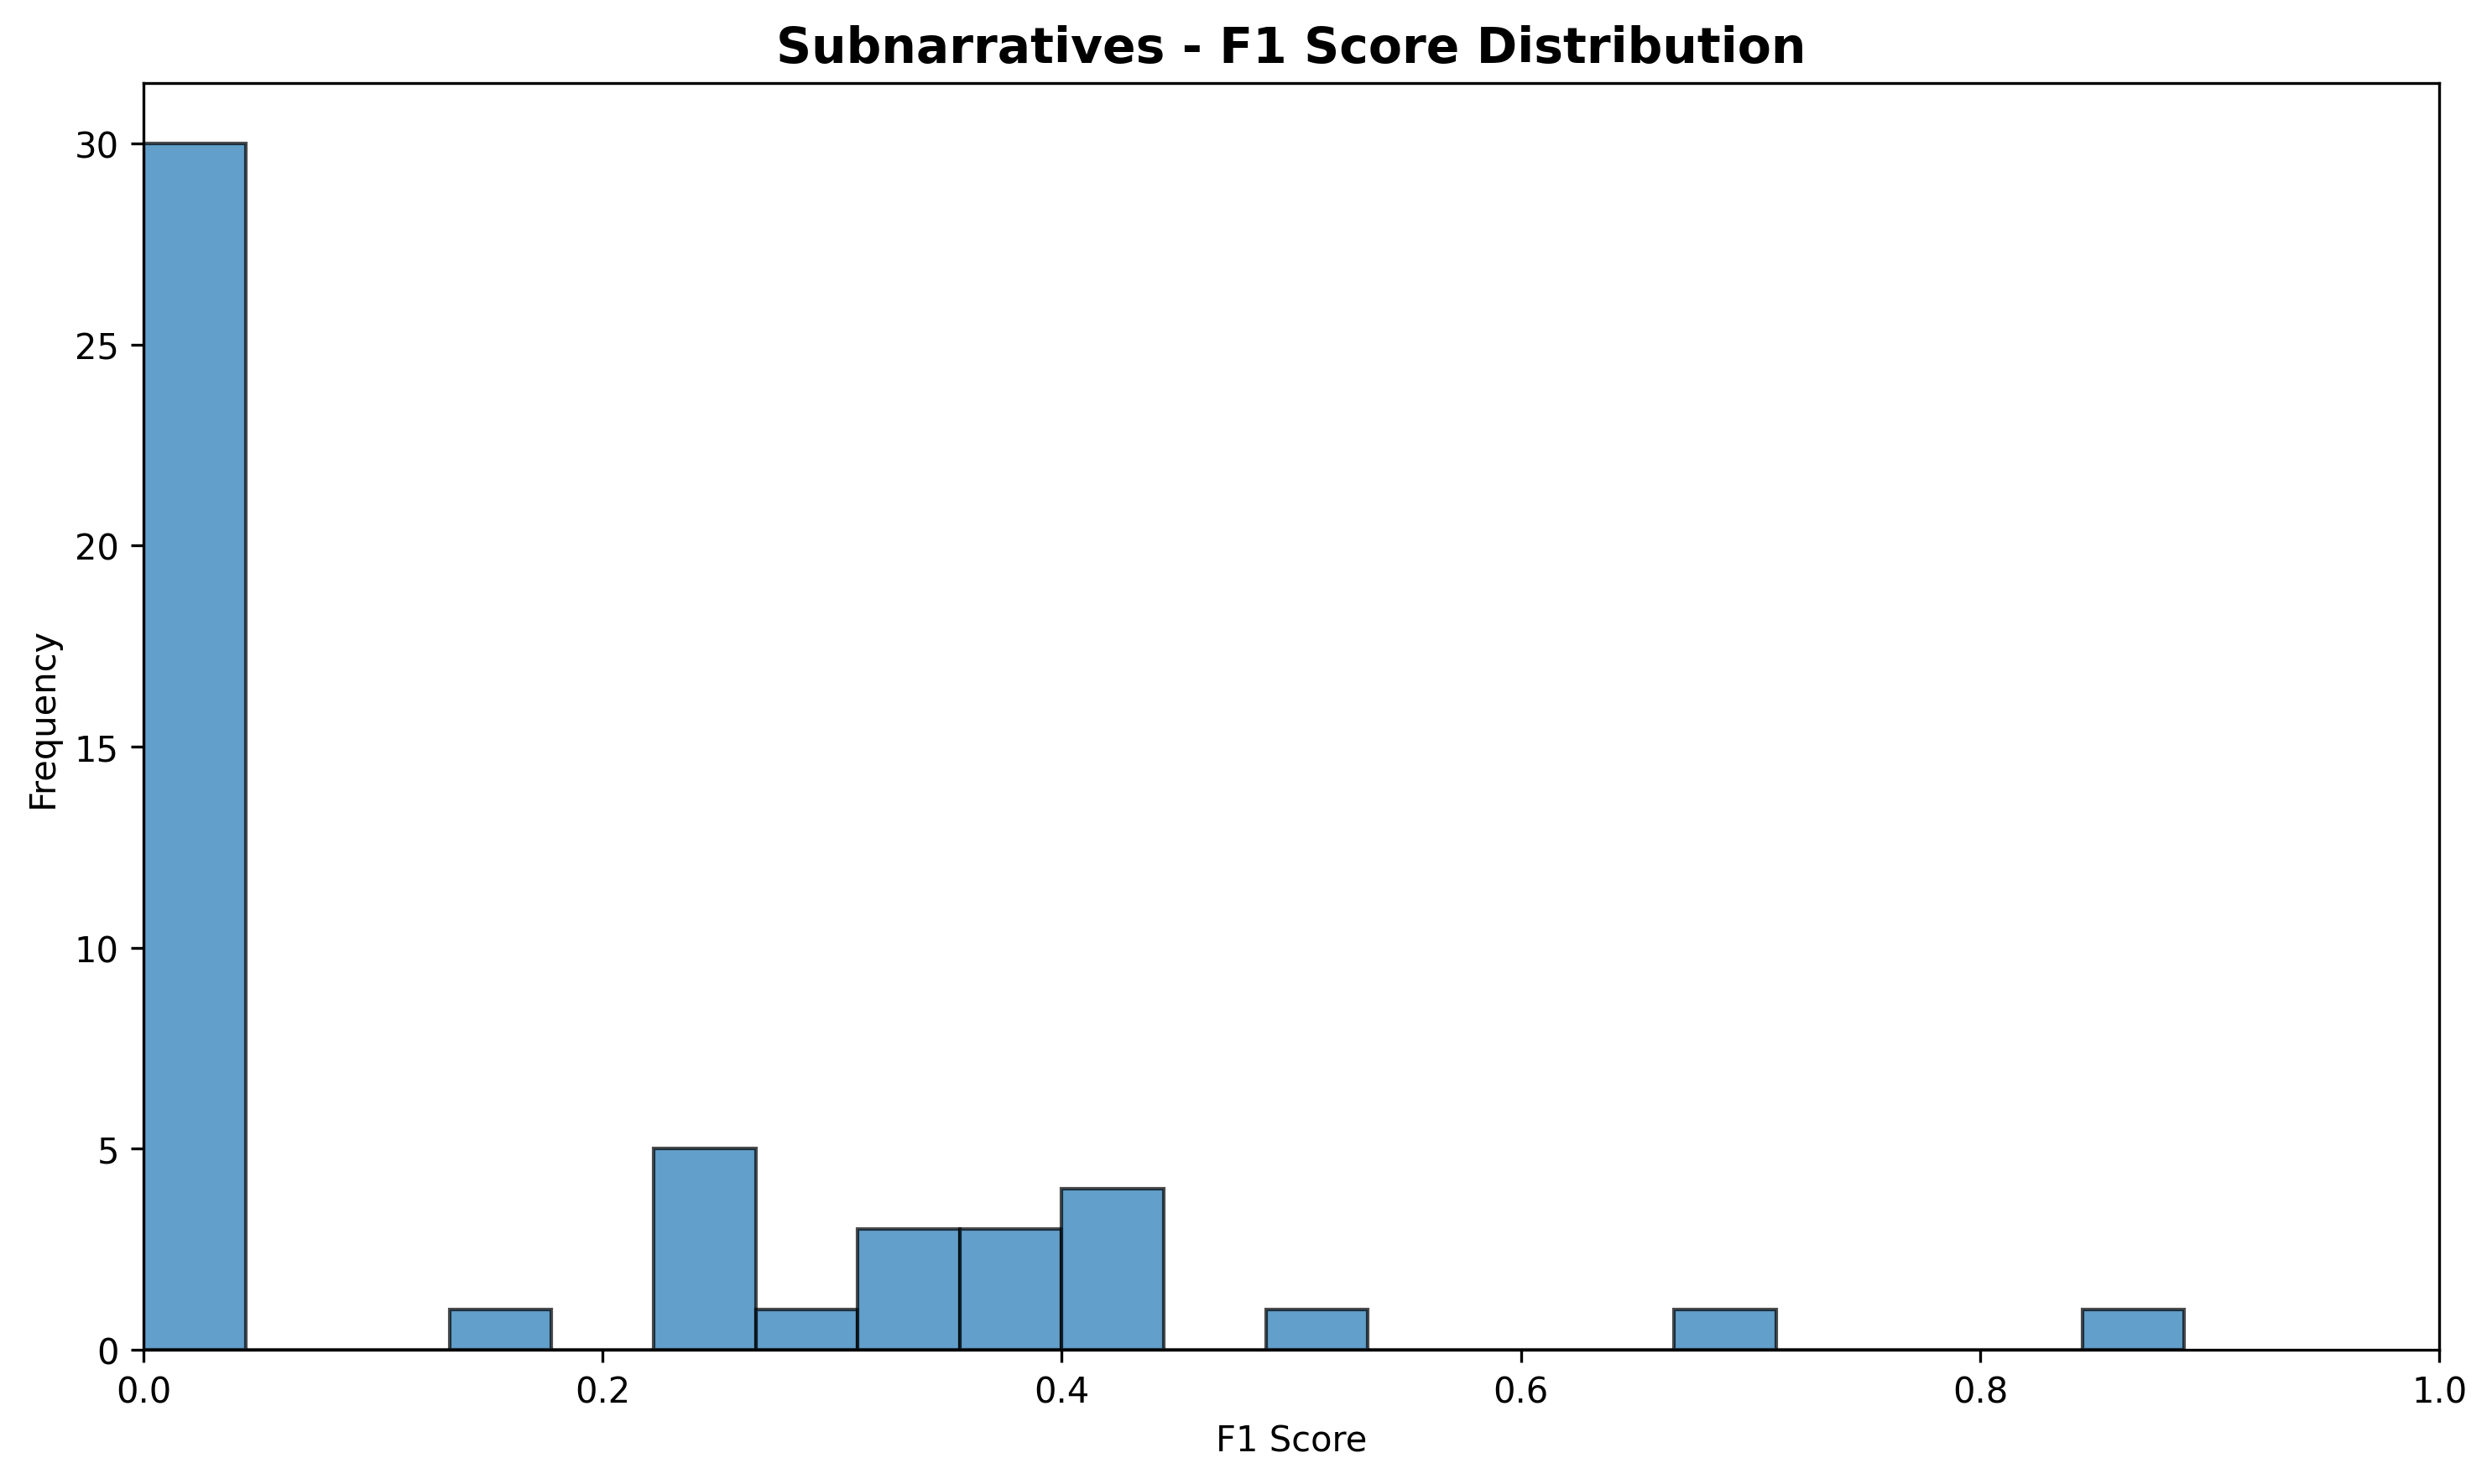
\includegraphics[width=\textwidth]{images/threshold_analysis/plots/subnarratives/f1_score_distribution.png}
        \caption{Subnarrative F1 score distribution}
        \label{fig:subnarratives-distribution}
    \end{subfigure}
    \caption{Subnarrative classification performance analysis at optimal threshold (0.7). (a) reveals significant language-specific challenges, particularly for Hindi. (b) shows the severely skewed F1 distribution, with most subnarratives achieving very low performance due to data scarcity.}
    \label{fig:subnarratives-detailed-analysis}
\end{figure}

\begin{figure}[htbp]
    \centering
    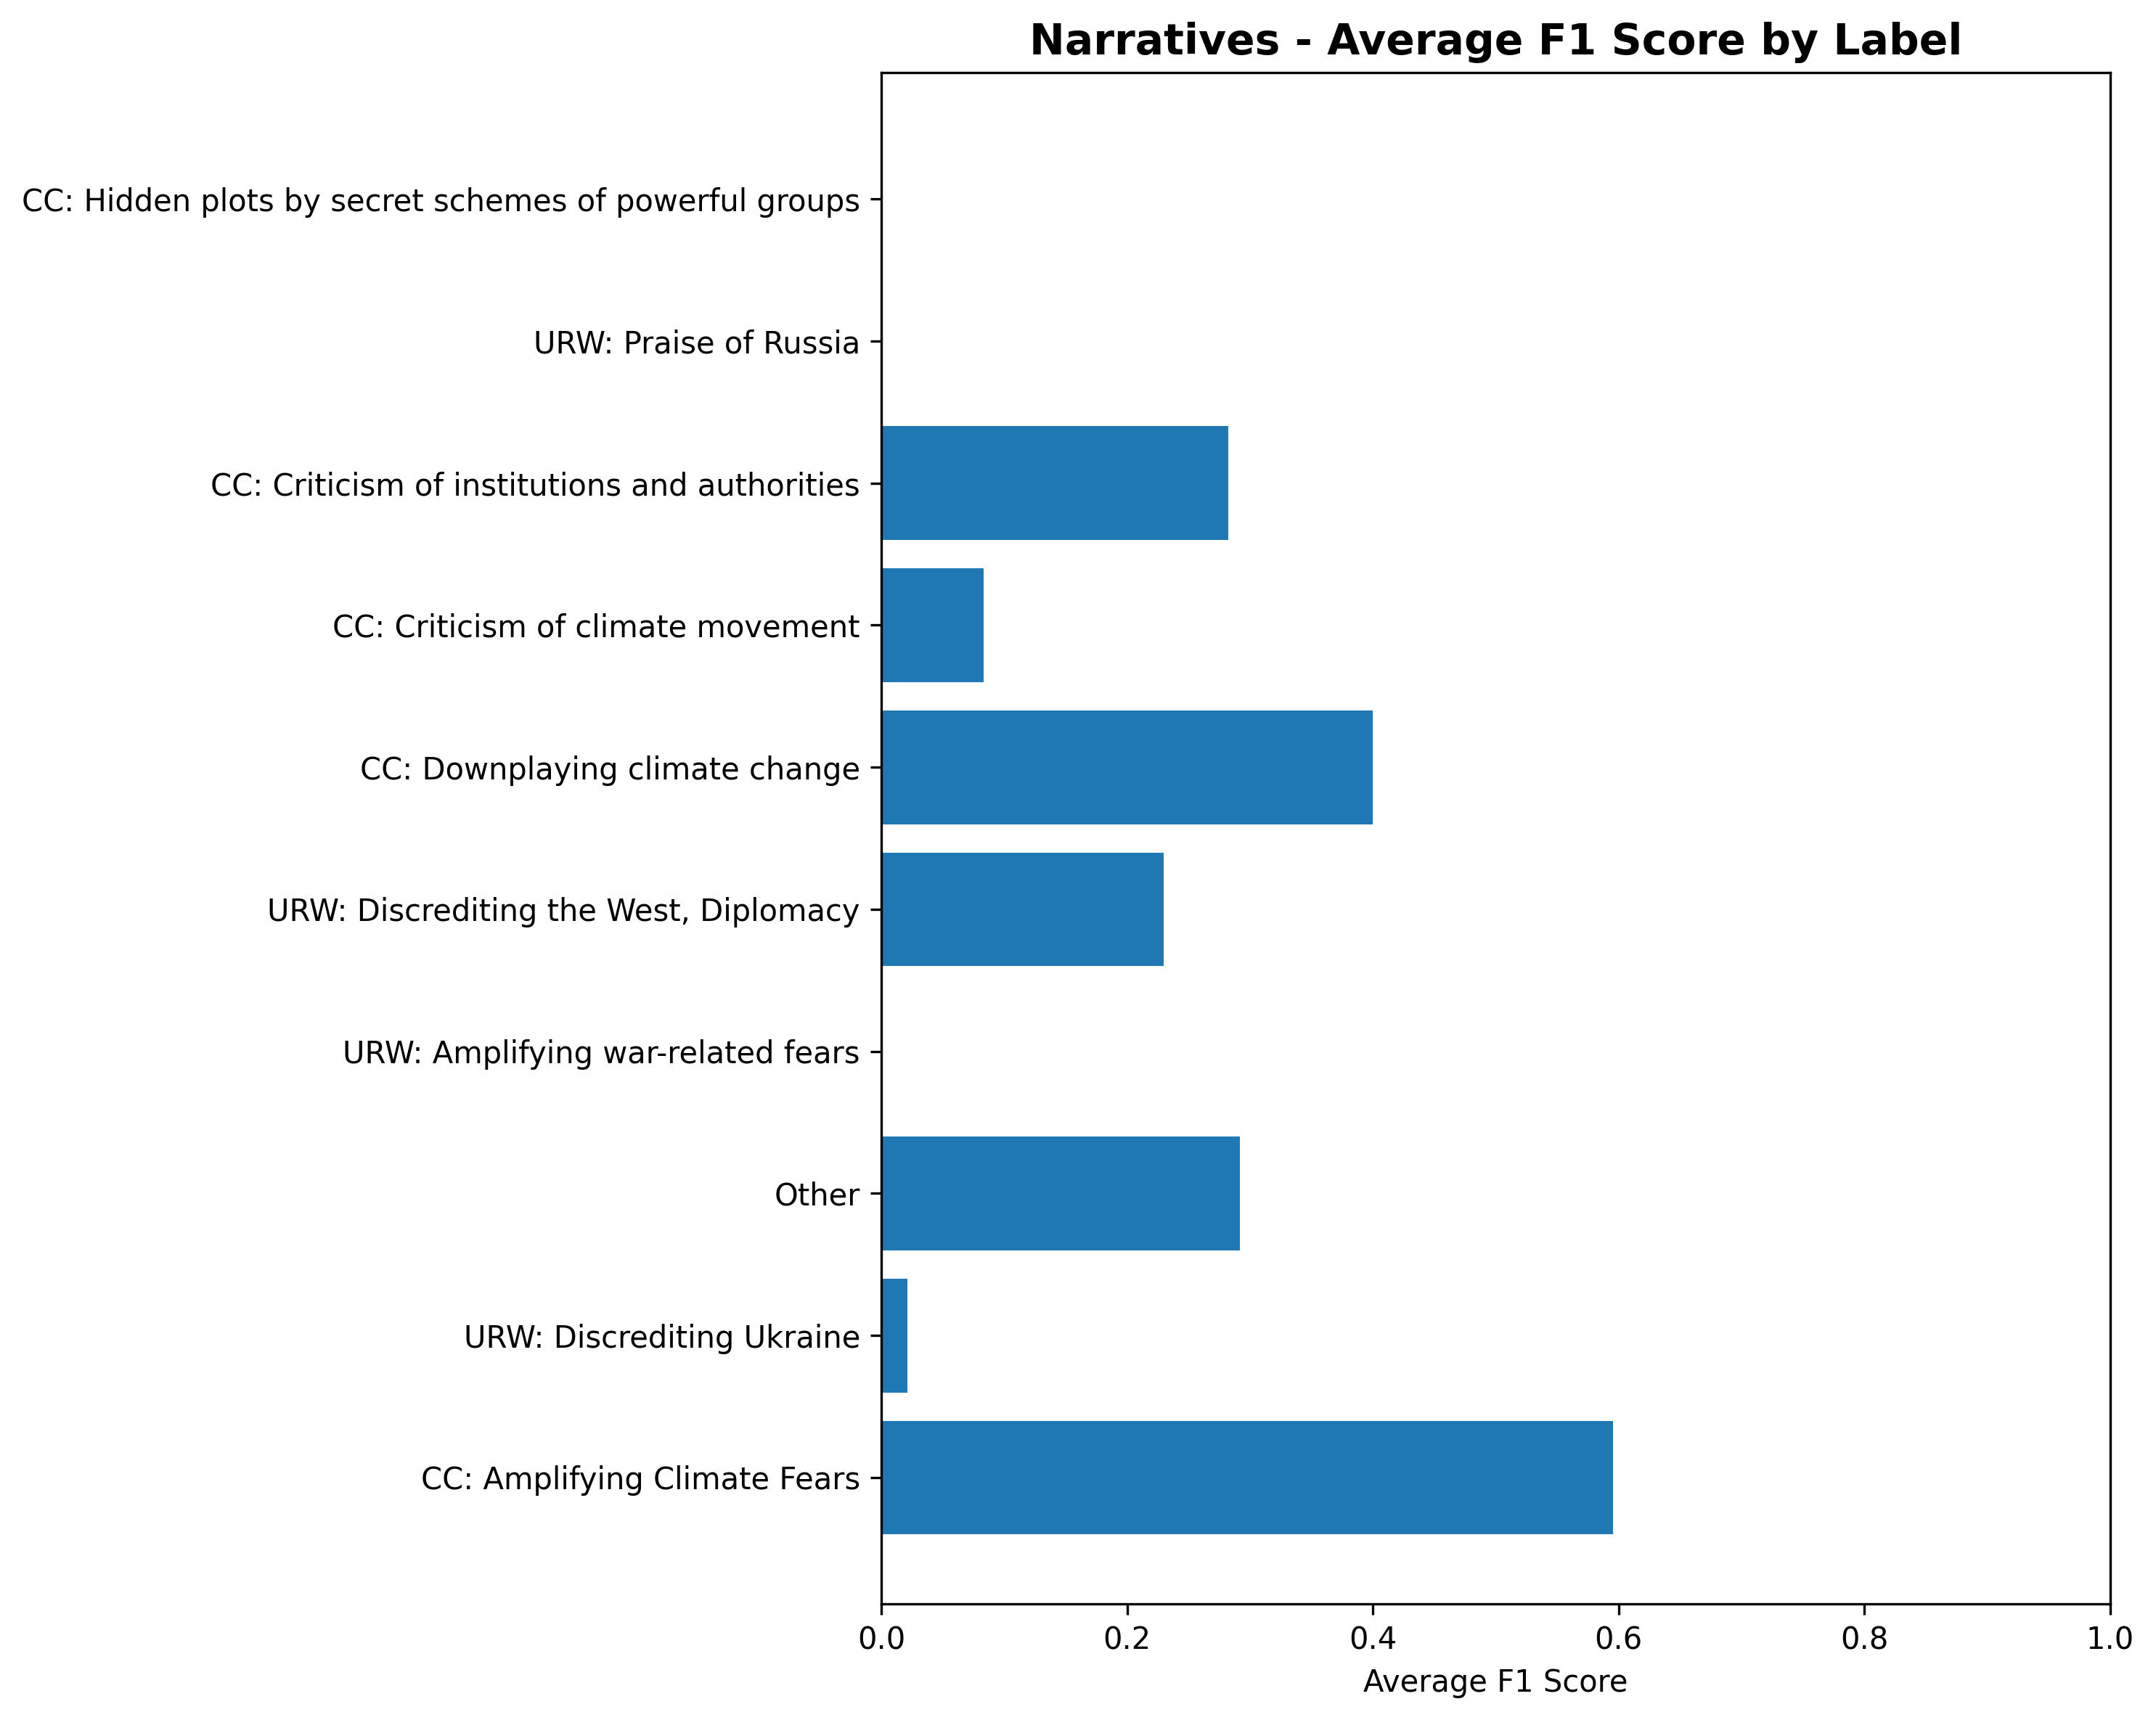
\includegraphics[width=0.9\textwidth]{images/threshold_analysis/plots/narratives/f1_score_by_label.png}
    \caption{F1 scores for individual narrative categories at threshold 0.65. Climate change narratives (CC:) generally outperform Ukraine-Russia war narratives (URW:), with ``CC: Questioning measurements and science'' achieving the highest performance. The substantial variation across categories highlights the impact of class imbalance and linguistic complexity.}
    \label{fig:narratives-by-label}
\end{figure}

\subsubsection{Hierarchical performance characteristics}

The substantial performance gap between narrative and subnarrative classification (F1 Samples: 0.2901 vs 0.1750 at optimal thresholds) illustrates the fundamental challenge of hierarchical classification. Even when using the optimal threshold for each level (0.65 for narratives, 0.8 for subnarratives), the fine-grained classification achieves only 60\% of the coarse-grained performance. Several factors contribute to this pattern:

\begin{itemize}
    \item \textbf{Data scarcity amplification}: Subnarratives inherit the data scarcity of their parent narratives and further subdivide the already limited examples
    \item \textbf{Increased semantic similarity}: Subnarratives within the same parent category often share similar linguistic features, making discrimination more challenging
    \item \textbf{Threshold sensitivity}: The different optimal thresholds suggest that the two classification levels require different decision boundaries
\end{itemize}

\subsection{Language-specific performance analysis}

Table~\ref{tab:language-performance} presents the performance breakdown by language using the optimal thresholds for each task level.

\begin{table}[htbp]
\centering
\caption{Language-specific performance using optimal thresholds (0.65 for narratives, 0.7 for subnarratives F1 Macro).}
\label{tab:language-performance}
\begin{tabular}{lcccc}
\toprule
\textbf{Language} & \multicolumn{2}{c}{\textbf{Narratives (0.65)}} & \multicolumn{2}{c}{\textbf{Subnarratives (0.7)}} \\
\cmidrule(lr){2-3} \cmidrule(lr){4-5}
& \textbf{F1 Macro} & \textbf{Best Threshold} & \textbf{F1 Macro} & \textbf{Best Threshold} \\
\midrule
Portuguese (PT) & \textbf{0.243} & 0.65 & \textbf{0.104} & 0.7 \\
English (EN) & 0.212 & 0.5 & 0.101 & 0.65 \\
Bulgarian (BG) & 0.209 & 0.7 & 0.080 & 0.7 \\
Russian (RU) & 0.170 & 0.65/0.5 & 0.095 & 0.7 \\
Hindi (HI) & \textbf{0.167} & 0.65 & 0.032 & 0.5 \\
\bottomrule
\end{tabular}
\end{table}

\paragraph{Portuguese demonstrates superior performance.} Portuguese achieves the highest F1 Samples scores for both narratives (0.352) and subnarratives (0.189), suggesting that the model learned particularly effective representations for Portuguese text. This represents a substantial 60\% advantage over the lowest-performing language (Hindi: 0.220 for narratives), highlighting significant cross-linguistic performance variation.

\paragraph{Hindi presents unique challenges.} Hindi shows the most substantial performance challenges, particularly evident in the F1 Samples scores. For narratives, Hindi achieves only 0.220 compared to Portuguese's 0.352, and for subnarratives, the gap is even more pronounced. This suggests that the model struggles with Hindi text across all levels of granularity, possibly due to linguistic complexity or limited training data quality.

\paragraph{Cross-linguistic performance patterns.} The F1 Samples results reveal that while threshold 0.8 optimizes subnarrative performance overall, language-specific patterns emerge. Russian shows surprisingly strong subnarrative F1 Samples performance (0.225), nearly matching narrative performance (0.245), suggesting that conservative thresholds particularly benefit Russian text classification.

\subsection{Detailed performance analysis at optimal threshold}

Using the optimal threshold of 0.65, we conducted detailed confusion matrix analysis to understand the model's strengths and limitations.

\subsubsection{Top-performing narrative categories}

Table~\ref{tab:top-narratives} shows the best-performing narrative categories, revealing clear patterns in what the model learned effectively.

\begin{table}[htbp]
\centering
\caption{Top 8 performing narrative categories at threshold 0.65, ranked by F1 score.}
\label{tab:top-narratives}
\begin{tabular}{lccccc}
\toprule
\textbf{Narrative Category} & \textbf{TP} & \textbf{FP} & \textbf{FN} & \textbf{Precision} & \textbf{F1} \\
\midrule
CC: Questioning measurements/science & 4 & 3 & 0 & 0.571 & \textbf{0.727} \\
CC: Criticism of climate policies & 6 & 2 & 3 & 0.750 & \textbf{0.706} \\
CC: Amplifying Climate Fears & 17 & 6 & 19 & 0.739 & \textbf{0.576} \\
URW: Discrediting the West, Diplomacy & 24 & 19 & 20 & 0.558 & \textbf{0.552} \\
CC: Criticism of institutions/authorities & 15 & 24 & 4 & 0.385 & \textbf{0.517} \\
CC: Downplaying climate change & 3 & 6 & 1 & 0.333 & \textbf{0.462} \\
URW: Discrediting Ukraine & 19 & 33 & 14 & 0.365 & \textbf{0.447} \\
CC: Criticism of climate movement & 6 & 13 & 3 & 0.316 & \textbf{0.429} \\
\bottomrule
\end{tabular}
\end{table}

\paragraph{Climate change narratives show strong performance.} The model demonstrates particular effectiveness in identifying climate change-related narratives, with 5 out of 8 top performers belonging to this domain. "CC: Questioning measurements/science" achieves perfect recall (1.000) and the highest F1 score (0.727), suggesting clear linguistic markers for scientific skepticism.

\paragraph{Precision-recall trade-offs vary by category.} "CC: Criticism of climate policies" achieves high precision (0.750) with moderate recall, while "CC: Criticism of institutions/authorities" shows the opposite pattern (precision: 0.385, recall: 0.789). This indicates that different narrative types have varying degrees of linguistic distinctiveness.

\subsubsection{Challenging categories and error analysis}

The bottom-performing categories reveal systematic challenges:

\begin{itemize}
    \item \textbf{URW: Negative Consequences for the West} (F1: 0.216): High false positive rate (25 FP vs 4 TP) suggests the model over-generalizes this category
    \item \textbf{URW: Blaming the war on others} (F1: 0.205): Low precision (0.167) indicates difficulty distinguishing from related war narratives
    \item \textbf{Other category} (F1: 0.233): The implicit negative classification strategy shows limited effectiveness
\end{itemize}

\subsubsection{Subnarrative classification challenges}

Subnarrative classification reveals the granularity limitations of the transformer approach:

\begin{itemize}
    \item \textbf{Best performer}: "CC: Amplifying Climate Fears: Amplifying existing fears" (F1: 0.640) demonstrates that some fine-grained distinctions are learnable
    \item \textbf{Systematic failures}: Many subnarratives achieve F1 scores below 0.300, indicating insufficient training data or overly subtle distinctions
    \item \textbf{Hindi-specific challenges}: Multiple subnarratives in Hindi achieve 0.000 F1 scores, suggesting language-specific modeling difficulties
\end{itemize}

\subsection{Key insights and limitations}

\subsubsection{Hierarchical classification challenges}

The substantial performance gap between narrative (F1 Samples: 0.2901) and subnarrative classification (F1 Samples: 0.1750 at optimal threshold 0.8) illustrates fundamental limitations of the fine-tuning approach for hierarchical tasks with limited data. Even with optimal threshold selection for each level, subnarratives achieve only 60\% of the narrative-level performance when evaluated on a per-document basis. The model successfully learns coarse-grained narrative patterns but struggles with fine-grained distinctions, particularly in low-resource languages.

\subsubsection{Language-specific patterns}

The significant variation in F1 Samples performance across languages (Portuguese: 0.352 vs Hindi: 0.220 for narratives) suggests that multilingual performance is not uniform. This 60\% performance gap indicates that the model's effectiveness varies substantially based on language, potentially reflecting differences in training data quality, linguistic complexity, or the effectiveness of the translation-based data augmentation strategy across different language pairs.

\subsubsection{Implications for system design}

These results provide crucial insights for the development of more advanced architectures:

\begin{itemize}
    \item \textbf{Threshold optimization} should be performed separately for each level of the hierarchy
    \item \textbf{Language-specific tuning} may be necessary for production deployment
    \item \textbf{Data augmentation strategies} beyond translation may be required for fine-grained classification
    \item \textbf{Alternative paradigms} (zero-shot, few-shot) warrant investigation given the limitations observed in the fine-tuning approach
\end{itemize}
